\begin{frame}[parent={cmap:software-testing-foundations}, hasprev=false, hasnext=true]
\frametitle{Falhas}
\label{concept:defect}

\begin{block:fact}{Produtos com falhas}
\begin{itemize}
    \item Nenhum produto é livre de falhas.
    \begin{itemize}
		\item E isso se aplica para qualquer tipo de produto, seja software ou hardware
    \end{itemize}
\end{itemize}

\hfill
\refie{example:produtos-com-falhas}{\beamerbutton{Example: Produtos com falhas}}
\end{block:fact}


\begin{block:fact}{Software com falhas}
\begin{itemize}
	\item Nenhum módulo de software é livre de falhas quando implementado e somente 40\% dos módulos de software são livres falhas quando liberado~\cite{shull-etal:2002}.
\end{itemize}
\hfill
\refie{example:falhas-de-software}{\beamerbutton{Example: Falhas de software}}
\end{block:fact}
\end{frame}


\begin{frame}[hasprev=true, hasnext=true]
\frametitle{Falhas}
\label{concept:defect-detection}

\begin{block:fact}{Todos os sofwates possuem falhas}
\begin{itemize}
	\item Mesmo softwares pequenos, simples e triviais são propensos a erros.
\end{itemize}
\end{block:fact}

\begin{block}{Example: Triângulo}
\centering
\refie{example:triângulos}{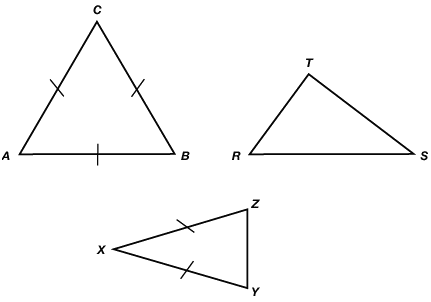
\includegraphics[scale=.5]{teste-de-software/conceitos-basicos/Imagens/triangulo-equilatero-isosceles-escaleno}}
\end{block}
\end{frame}


\begin{frame}[hasprev=true, hasnext=false]
\frametitle{Falhas}

\begin{block:fact}{Evitar e detectar falhas}
\begin{itemize}
	\item No entanto, produtos com falhas podem e devem ser evitados e corrigidos, uma vez que afeta negativamente a qualidade do software
\end{itemize}
\end{block:fact}


\begin{block:fact}{Por que devemos nos preocupar com isso?}
\begin{itemize}
    \item A crescente demanda por maior qualidade de software

    \item A redução de falhas no software melhora sua qualidade.
\end{itemize}
\end{block:fact}

\begin{block:fact}{Qualidade e teste de software}
\begin{itemize}
	\item O principal objetivo do teste de software é encontrar falhas.

	\item Testes de softwares sistemáticos, realizada utilizando técnicas adequadas, critérios e ferramentas, melhora a confiabilidade do software (e qualidade).
\end{itemize}
\end{block:fact}
\end{frame}
